\section*{Figure and tables}

\begin{figure*}[htb]
%\captionsetup{justification=centering, font=footnotesize}
\vspace{-2em}
\begin{center}
\subfigure[]{\epsfxsize=0.31\linewidth \epsfbox{depthplot_cropped}}
\subfigure[]{\epsfxsize=0.31\linewidth \epsfbox{penalties1}}
\subfigure[]{\epsfxsize=0.31\linewidth \epsfbox{threslarn}}
\vspace{-1em}
\caption{(a) Surface and contours of a data depth function for bivariate normal distribution; (b) Comparison of L1 and SCAD \citep{FanLi01} penalty functions with depth at a scalar point: inverting the depth function helps obtain the nonconvex shape of the penalty function in the inverse depth; (c) Univariate thresholding rule for the LARN estimate (see section \ref{sec:sec4})}
\label{fig:fig1}
\end{center}
\end{figure*}

\begin{figure*}[h]
%\captionsetup{justification=centering, font=footnotesize}
\begin{center}
%\subfigure[]{\epsfxsize=0.31\linewidth \epsfbox{../../Codes/plot1log}}
%\subfigure[]{\epsfxsize=0.31\linewidth \epsfbox{../../Codes/plot2log}}
%\subfigure[]{\epsfxsize=0.31\linewidth \epsfbox{../../Codes/plot3log}}\\
\subfigure[]{\epsfxsize=0.31\linewidth \epsfbox{plot1mspe}}
\subfigure[]{\epsfxsize=0.31\linewidth \epsfbox{plot2mspe}}
\subfigure[]{\epsfxsize=0.31\linewidth \epsfbox{plot3mspe}}

\caption{Mean absolute Estimation Errors for all three methods in different $(p,q)$ settings}
\label{fig:simplots}
\end{center}
\end{figure*}

\begin{figure*}[t]
%\captionsetup{justification=centering, font=footnotesize}
\begin{center}
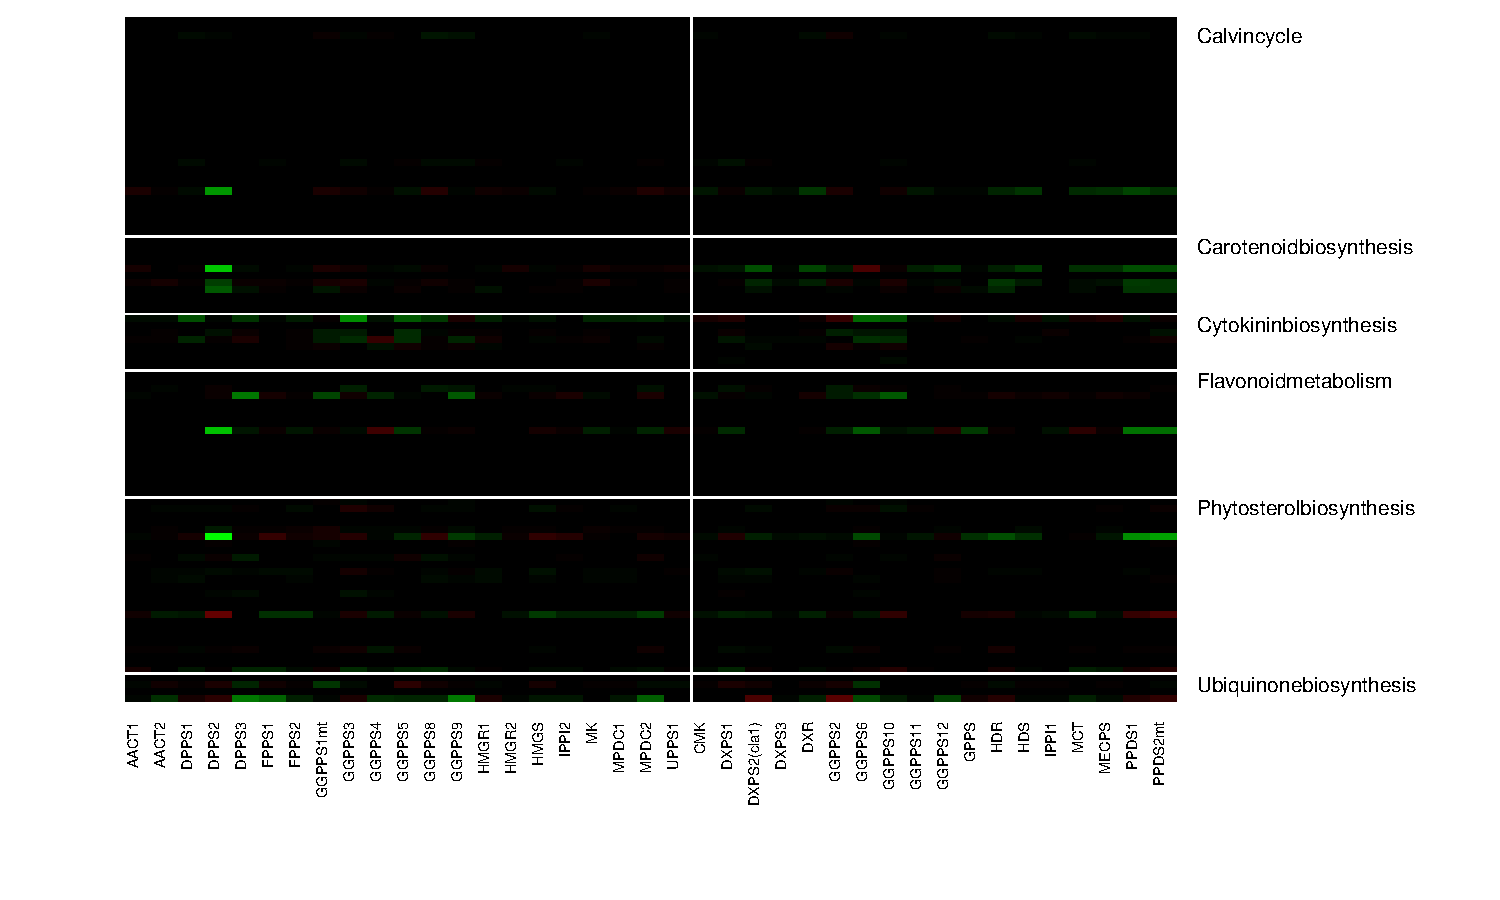
\includegraphics[width=\textwidth]{cropped_gene_heatmap1}

\caption{Estimated effects of different pathway genes on the activity of genes in Mevalonate and Non-mevalonate pathways (left and right of vertical line) in \textit{A. thaliana}}
\label{fig:coeffplots}
\end{center}
\end{figure*}
%

%
\begin{table}[t]
\centering
\begin{small}
    \caption{Average true positive and true negative (TP/TN) rates for 3 methods, for $n=50$ and AR1 covariance structure}
    \vspace{.1in}
    \begin{tabular}{c|ccc}
    \hline
    $\rho$ & GL-t & SGL       & LARN      \\ \hline
    \multicolumn{4}{l}{ (a) $p=20, q=20$}\\\hline
    0.9               & 0.77/0.83          & 0.92/0.99 & 0.91/0.92 \\
    0.7               & 0.81/0.83          & 0.91/0.99 & 0.89/0.93 \\
    0.5               & 0.78/0.79          & 0.89/0.99 & 0.88/0.92 \\
    0.0               & 0.85/0.78          & 0.90/0.99 & 0.90/0.91 \\ \hline
    \multicolumn{4}{l}{ (b) $p=20, q=60$}\\\hline
    0.9               & 0.90/0.66          & 0.95/0.97 & 0.89/0.92 \\
    0.7               & 0.91/0.70          & 0.93/0.96 & 0.90/0.92 \\
    0.5               & 0.80/0.69          & 0.94/0.98 & 0.93/0.92 \\
    0.0               & 0.85/0.68          & 0.93/0.97 & 0.91/0.92 \\ \hline
    \multicolumn{4}{l}{ (c) $p=60, q=60$}\\\hline
    0.9               & 0.57/0.79          & 0.68/0.99 & 0.85/0.93 \\
    0.7               & 0.50/0.79          & 0.64/0.99 & 0.83/0.93 \\
    0.5               & 0.54/0.81          & 0.64/0.99 & 0.85/0.93 \\
    0.0               & 0.58/0.79          & 0.63/0.99 & 0.84/0.93 \\ \hline
    \end{tabular}
        \end{small}
    \label{table:simtable2}
\end{table}

\begin{table}[t]
\centering
    \caption{Total runtimes in seconds for SGL and LARN algorithms for the three simulation settings}
    \vspace{.1in}
    \begin{tabular}{c|ccc}
    \hline
    Setting & GL-t & SGL    & LARN \\ \hline
    (a)     & 332 & 490    & 209  \\
    (b)       & 676 & 52  & 328 \\
    (c)       & 4994 & 39760 & 3883 \\ \hline
    \end{tabular}
    \label{table:simtimetable}
\end{table}

% latex table generated in R 3.2.4 by xtable 1.8-2 package
% Sun Oct 02 19:29:30 2016
\begin{table}[htb]
\centering
\begin{small}
\begin{tabular}{rll}
  \hline
Coeff & Gene & Pathway \\ 
  \hline
0.18 & DPPS2 & Phytosterol biosynthesis \\ 
0.14 & DPPS2 & Carotenoid biosynthesis \\ 
0.14 & DPPS2 & Flavonoid metabolism \\ 
0.11 & DPPS2 & Calvin cycle \\ 
0.11 & PPDS2mt & Phytosterol biosynthesis \\ 
0.10 & GGPPS3 & Cytokinin biosynthesis \\ 
0.10 & PPDS1 & Phytosterol biosynthesis \\ 
0.09 & DPPS3 & Flavonoid metabolism \\ 
0.09 & DPPS3 & Ubiquinone biosynthesis \\ 
0.09 & GGPPS9 & Ubiquinone biosynthesis \\ 
\hline
\end{tabular}
\end{small}
\caption{Top 10 gene-pathway connections in {\it A. thaliana} data found by LARN}
\label{table:coefftable}
\end{table}
\vspace{5em}